\documentclass[12pt,a4paper]{report}

\usepackage[spanish]{babel}
\usepackage[T1]{fontenc}
\usepackage[utf8]{inputenc}
\usepackage{amsmath}
\usepackage{graphicx}
\usepackage[page]{appendix}
\usepackage{listings}
\usepackage{color}

\addto\captionsspanish{\renewcommand\appendixpagename{Archivos de código}}

\DeclareFixedFont{\ttb}{T1}{txtt}{bx}{n}{9}
\DeclareFixedFont{\ttm}{T1}{txtt}{m}{n}{9} 
\DeclareFixedFont{\tti}{T1}{txtt}{m}{it}{9}
\definecolor{comment}{RGB}{150,150,150}

\lstset{
	frame = single, 
	extendedchars=true,	
	showstringspaces=false,
	inputencoding=utf8,
	literate={á}{{\'a}}1 {é}{{\'e}}1 {í}{{\'i}}1 {ó}{{\'o}}1 {ú}{{\'u}}1 {ñ}{{\~n}}1
	{Á}{{\'A}}1 {É}{{\'E}}1 {Í}{{\'I}}1 {Ó}{{\'O}}1 {Ú}{{\'U}}1 {Ñ}{{\~N}}1,
	language=Python,
	basicstyle=\ttm,
	otherkeywords={self},
	keywordstyle=\ttb,
	commentstyle=\tti\color{comment}
	}




% Indica el título del documento como la palabra "Práctica " seguida del número de práctica.
\title{Práctica 1}

% Indica tu nombre completo
\author{Javier Gálvez Obispo }

\begin{document}

\maketitle

\section*{Ejercicio 1}

% Incluye aquí el texto correspondiente al ejercicio 1

\noindent
Represente las posiciones de los puntos respecto de la trama \textbf{\{\textit{A}\}} cuando:
\renewcommand{\theenumi}{\alph{enumi}}
\begin{enumerate}
    \item La trama \textbf{\{\textit{B}\}} se gira un ángulo $\alpha = 90^\circ$ alrededor del eje $X_A$
    \item La trama \textbf{\{\textit{B}\}} se gira un ángulo $\alpha = 90^\circ$ alrededor del eje $Y_A$
    \item La trama \textbf{\{\textit{B}\}} se gira un ángulo $\alpha = 90^\circ$ alrededor del eje $Z_A$
\end{enumerate}
Interprete el resultado.\\

\noindent
En la siguiente figura se muestran los 3 giros junto a los puntos originales.

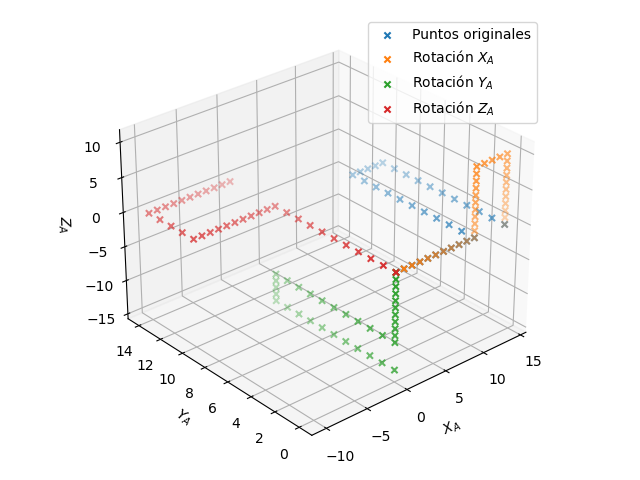
\includegraphics[]{Ejercicio_1.png}

\section*{Ejercicio 2}

Represente las posiciones de los puntos respecto de la trama \textbf{\{\textit{A}\}} cuando la trama \textbf{\{\textit{B}\}} del ejercicio anterior se rota desde la posición original (superpuesta a la trama \textbf{\{\textit{A}\}}) entorno al eje $X_B$ un ángulo $\gamma = 60^\circ$, a continuación se gira entorno al eje $Y_B$ un ángulo $\beta = 90^\circ$, y después se gira entorno al eje $Z_B$ un ángulo $\alpha = 30^\circ$. \\
Compruebe como afecta el orden de las rotaciones en las coordenadas respecto de la trama \textbf{\{\textit{A}\}}. Comente el resultado. \\

\noindent
El ejercicio nos indica que las rotaciones se hacen respecto a la trama en movimiento, es decir, utilizamos ángulos de Euler. Entonces, para calcular la matriz de rotación descrita $^AR_B$ multiplicamos las distintas matrices de rotación en el mismo orden que se indica en el enunciado $^AR_B = R(X_B, 60^\circ) \cdot R(Y_B, 90^\circ) \cdot R(Z_B, 30^\circ)$.\\
Para comprobar como afecta el orden de las rotaciones a las coordenadas de los puntos invertimos el orden de las matrices en el producto: $^AR_B = R(Z_B, 30^\circ) \cdot R(Y_B, 90^\circ) \cdot R(X_B, 60^\circ)$.\\
En la siguiente figura se puede comprobar los distintos resultados.

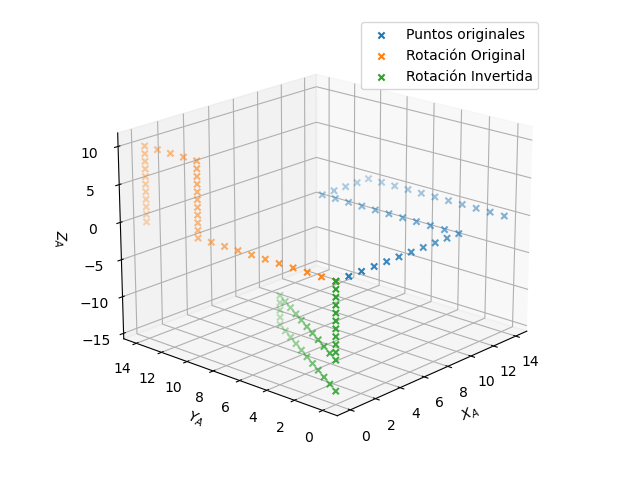
\includegraphics[]{Ejercicio_2.png}

\section*{Ejercicio 3}

% Usa tantas secciones como ejercicios haya y las subsecciones que necesites

Diseñe e implemente una función en Python que reciba como entrada una matriz de dimensión \textit{n} x 4 con los parámetros de Denavit-Hartenberg de un manipulador cualquiera, y devuelva como salida la matriz de transformación homogénea (como un array de dimensión 4 x 4) que relaciona el sistema de coordenas de la base y el sistema de coordenadas del extremo del robot. Contemple la posibilidad de que los ángulos de rotación y los desplazamientos sean variables simbólicas (use el paquete \textbf{sympy}). Compruebe el correcto funcionamiento de la función con algunos ejemplos.\\

\noindent
Para comprobar el correcto funcionamiento de la función se ha utilizado el ejemplo de la diapositiva 17 del tema 4 en el que los parámetros de Denavit-Hartenberg son los siguientes:

\begin{center}
\begin{tabular}{|c|c|c|c|c|}
    \hline
    \textit{i} & $\theta_i$ & $d_i$ & $a_i$ & $\alpha_i$ \\
    \hline
    1 & $q_1$ & $l_1$ & 0 & 0 \\
    \hline
    2 & $90^\circ$ & $q_2$ & 0 & $90^\circ$ \\
    \hline
    3 & 0 & $l_1 + q_3$ & 0 & 0 \\
    \hline
\end{tabular}
\end{center}
Además, este ejemplo también muestra como la función implementada puede trabajar indistintamente con valores numéricos y variables simbólicas.
La matriz que nos devuelve la función es la siguiente:\\

\noindent
Matrix([[-sin(q1), 0, cos(q1), (l3 + q3)*cos(q1)], [cos(q1), 0, sin(q1), (l3 + q3)*sin(q1)], [0, 1, 0, l1 + q2], [0, 0, 0, 1]])

\begin{center}
    $^0T_3 = 
    \begin{bmatrix}
        -sin(q_1) & 0 & cos(q_1) & (l_3 + q_3)*cos(q_1)\\
        cos(q_1) & 0 & sin(q_1) & (l_3 + q_3)*sin(q_1)\\
        0 & 0 & 1 & l_1 + q_2\\
        0 & 0 & 0 & 1\\
    \end{bmatrix}$ 
\end{center}
Es fácil comprobar el correcto funcionamiento comparando el resultado obtenido con la diapositiva 18 del tema 4 de la asignatura.


% Debes incluir todos los archivos de código de Python que hayas generado.
% Para ello introduce una sección por cada archivo dentro del entorno appendices
% Sigue el esquema que tienes a continuación donde el título de la sección debe
% coincidir con el nombre del archivo y mediante el comando \lstinputlisting
% añades el texto del archivo. Recuerda que las rutas de los archivos .m deben
% ser relativas a la ruta de este achivo .tex

\begin{appendices}
	\section*{ejercicio1.py}
	\lstinputlisting{ejercicio1.py}

	\section*{ejercicio2.py}
	\lstinputlisting{ejercicio2.py}

	\section*{ejercicio3.py}
	\lstinputlisting{ejercicio3.py}

	%Usa tantas secciones en el apéndice como archivos de código tengas.	
	
\end{appendices}

\end{document}
